\chapter{Skin Effect and Non-Bloch Light}
\label{ch:skin-effect}

\begin{chapterlead}
In Hermitian photonic crystals, Bloch's theorem guarantees that
eigenstates are extended plane waves modulated by a periodic function.
In non-Hermitian crystals, this guarantee can fail: under open
boundary conditions, an extensive fraction of the eigenstates can pile up
at one edge of the system. This is the \emph{non-Hermitian skin effect}
(NHSE), and it demands a complete rethinking of band theory. The wave
vector acquires an imaginary part, the Brillouin zone deforms into a
\emph{generalized Brillouin zone} (GBZ), and topological invariants must
be redefined on this new contour to restore the bulk-boundary
correspondence. The theory of the skin effect is developed from the
perspective of photonic systems, leading to the non-Bloch band theory
that replaces conventional Bloch analysis.
\end{chapterlead}


%% ================================================================
\section{The breakdown of Bloch band theory}
\label{sec:bloch-breakdown}

Consider a one-dimensional non-Hermitian photonic crystal of $L$ unit
cells with open boundary conditions. In a Hermitian system, the
eigenstates of such a finite chain approach extended Bloch waves as
$L \to \infty$, with eigenfrequencies tracing the bulk bands. In a
non-Hermitian system, the picture changes.

\subsection{Skin modes}
\label{ssec:skin-modes}

Numerical diagonalization of a simple skin-effect Hamiltonian reveals
that an extensive set of eigenstates---not just a few edge states, but
the bulk spectrum itself---can become exponentially localized at one
boundary of the chain. The localization length is finite and independent
of $L$ in the standard NHSE. This is the non-Hermitian skin effect: an
$O(L)$ number of states are boundary-localized, in contrast to the
$O(1)$ boundary states of Hermitian topological insulators.

\subsection{Spectral sensitivity}
\label{ssec:spectral-sensitivity}

The open-boundary spectrum can differ strongly from the
periodic-boundary (PBC) spectrum. Under PBC, the eigenfrequencies form
closed loops in the complex plane (the bands of
Chapter~\ref{ch:complex-bands}). Under open boundary conditions (OBC),
the spectrum collapses onto arcs or curves that bear little resemblance
to the PBC loops. Conventional Bloch-Hamiltonian invariants, computed
from the PBC spectrum, fail to predict the OBC physics---including the
presence or absence of topological zero modes.

\subsection{A quantitative measure}
\label{ssec:skin-quantitative}

The skin effect can be quantified by the inverse participation ratio
(IPR) or by the mean center of mass of the eigenstates. For an $L$-site
chain with eigenstate $|\psi_j\rangle$ and amplitudes $\psi_j(n)$ at
site $n$, the center of mass is
\begin{equation}
 \bar{n}_j = \sum_{n=1}^{L} n\,|\psi_j(n)|^2
 \bigg/ \sum_{n=1}^{L} |\psi_j(n)|^2.
 \label{eq:center-of-mass}
\end{equation}
In a Hermitian system, $\bar{n}_j \approx L/2$ for bulk states. In a
standard skin-effect system, $\bar{n}_j \to 1$ (or $\bar{n}_j \to L$)
for an extensive set of eigenstates, signaling macroscopic boundary
accumulation.

\begin{figure}[t]
 \centering
 
\includegraphics[width=0.72\textwidth]{fig_f14_pbc_obc_spectra.pdf}
 \caption{The non-Hermitian skin effect announces itself through spectral
 sensitivity to boundary conditions~\cite{hatano1996localization}. In the Hatano--Nelson toy model, the
 periodic-boundary spectrum forms a complex loop, while the open-boundary
 spectrum collapses onto the non-Bloch/GBZ prediction~\cite{yao2018edge,yokomizo2019non}. This is the
 computational signature behind the failure of ordinary Bloch
 bulk-boundary correspondence.}
 \label{fig:skin-pbc-obc-spectra}
\end{figure}

\begin{figure}[t]
 \centering
 
\includegraphics[width=0.95\textwidth]{fig_f14_skin_modes.pdf}
 \caption{Skin modes are not a small number of edge states; in the
 standard NHSE an extensive fraction of the open-chain eigenvectors
 accumulates near one boundary. The plotted representative normalized
 eigenmode intensities decay exponentially away from the accumulation
 edge on a logarithmic scale.}
 \label{fig:skin-mode-localization}
\end{figure}


%% ================================================================
\section{Physical origin of the skin effect}
\label{sec:skin-origin}

The skin effect arises when non-Hermiticity produces a nonzero
point-gap winding, most transparently through \emph{asymmetric} coupling
between sites. In a tight-binding picture, if the hopping amplitude from
left to right ($t_R$) differs from right to left ($t_L$), a particle is
preferentially transported in one direction, and eigenstates accumulate
at the corresponding boundary. Asymmetric hopping is the cleanest route,
but the more general diagnostic is the boundary-sensitive point-gap
spectrum discussed in Chapter~\ref{ch:point-gap}.

\subsection{Sources of asymmetry in photonic systems}
\label{ssec:asymmetry-sources}

In photonic systems, this asymmetry can arise from:
\begin{itemize}
 \item \textbf{Non-reciprocal elements:} magneto-optical materials or
 active components that break Lorentz reciprocity.
 \item \textbf{Engineered gain/loss reservoirs:} auxiliary lossy or
 amplifying paths that produce direction-dependent effective coupling
 after unobserved channels are eliminated.
 \item \textbf{Coupled-resonator networks:} auxiliary coupling paths
 that make the reduced modal hopping asymmetric. A reciprocal
 full-wave device may still have a symmetric scattering matrix; the
 nonreciprocity here is an effective description of a selected
 subsystem.
 \item \textbf{Time modulation:} periodic temporal modulation of the
 refractive index that breaks time-reversal symmetry and creates
 effective non-reciprocal hopping in the Floquet picture.
\end{itemize}

\subsection{The imaginary gauge field}
\label{ssec:imaginary-gauge}

The mathematical signature of the skin effect is that the eigenvalues
$\beta = e^{ik}$ of the transfer matrix (or the Bloch phase factor) are
no longer on the unit circle $|\beta| = 1$. Instead, they satisfy
$|\beta| = r \neq 1$, corresponding to an exponentially growing or
decaying spatial profile. The wave vector acquires an imaginary part:
$k \to k - i\kappa_{\mathrm{skin}}$, where
$\kappa_{\mathrm{skin}} = \ln r$ is the skin decay constant.

This can be understood as an \emph{imaginary gauge field}~\cite{longhi2019probing,zhang2021observation,yang2020non,yang2026non}: the
asymmetric hopping is equivalent to a uniform imaginary vector
potential. Under OBC the asymmetry can be removed from the Hatano--Nelson
Hamiltonian by a non-unitary similarity transform, but the transformed
back eigenvectors acquire an exponential envelope. Under PBC the same
transform changes the boundary condition by a complex flux, so the
asymmetry remains visible in the periodic spectrum as a complex loop.
This gauge-theoretic perspective explains why the PBC and OBC spectra
are so different.


%% ================================================================
\section{Example: the Hatano--Nelson model}
\label{sec:hatano-nelson}

The Hatano--Nelson model is the simplest system that exhibits the skin
effect. It is a one-dimensional tight-binding chain with asymmetric
nearest-neighbor hopping:
\begin{equation}
 H = \sum_{n=1}^{L-1}\bigl(t_R\,|n\rangle\langle n+1|
 + t_L\,|n+1\rangle\langle n|\bigr),
 \label{eq:hn-hamiltonian}
\end{equation}
with $t_R \neq t_L$ and $t_R, t_L > 0$.

\subsection{PBC spectrum}
\label{ssec:hn-pbc}

Under periodic boundary conditions, the Bloch Hamiltonian is
\begin{equation}
 H(k) = t_R\,e^{ik} + t_L\,e^{-ik},
 \label{eq:hn-bloch}
\end{equation}
and the eigenvalues trace an ellipse in the complex plane:
\begin{equation}
 E_{\mathrm{PBC}}(k) = (t_R + t_L)\cos k + i(t_R - t_L)\sin k,
 \label{eq:hn-pbc-spectrum}
\end{equation}
with semi-major axis $t_R + t_L$ and semi-minor axis $|t_R - t_L|$. The
spectral winding number (Section~\ref{sec:winding}) around any point
inside the ellipse is $\wnum = +1$ (for $t_R > t_L$).

\subsection{OBC spectrum}
\label{ssec:hn-obc}

Under open boundary conditions, the spectrum collapses onto the real
interval $[-2\sqrt{t_R t_L},\; 2\sqrt{t_R t_L}]$. In this model the
PBC ellipse collapses
onto a line segment. All eigenvalues are real, and all right eigenstates
localize at the left boundary (for $t_R > t_L$).  The amplitude envelope
is controlled by the GBZ radius,
\begin{equation}
  |\psi_n| \propto r_{\mathrm{GBZ}}^{\,n},\qquad
  r_{\mathrm{GBZ}}=\sqrt{\frac{t_L}{t_R}},
  \label{eq:hn-localization}
\end{equation}
so the amplitude localization length is
$\xi_{\mathrm{amp}}=1/|\ln r_{\mathrm{GBZ}}|=2/\ln(t_R/t_L)$.  If one
fits the intensity $|\psi_n|^2$ instead, the corresponding intensity
length is $\xi_{\mathrm{int}}=\xi_{\mathrm{amp}}/2=1/\ln(t_R/t_L)$.
We will state explicitly which convention is being used whenever a
localization length is quoted.

\subsection{GBZ construction}
\label{ssec:hn-gbz}

The GBZ for the Hatano--Nelson model can be found analytically. Replace
$e^{ik}$ by $\beta$ in~\eqref{eq:hn-bloch}:
$H(\beta) = t_R\beta + t_L/\beta$. The characteristic equation
$H(\beta) = E$ gives a quadratic in $\beta$:
\begin{equation}
 t_R\beta^2 - E\beta + t_L = 0,
 \label{eq:hn-characteristic}
\end{equation}
with two solutions $\beta_1, \beta_2$ satisfying
$\beta_1\beta_2 = t_L/t_R$. The GBZ condition
$|\beta_1| = |\beta_2|$ gives
\begin{equation}
 |\beta|^2 = \frac{t_L}{t_R}
 \quad\Longrightarrow\quad
 |\beta| = \sqrt{\frac{t_L}{t_R}} \equiv r_{\mathrm{GBZ}}.
 \label{eq:hn-gbz-radius}
\end{equation}
The GBZ is a circle of radius $r_{\mathrm{GBZ}} < 1$ (for $t_R > t_L$)
centered at the origin in the complex $\beta$ plane.

\begin{figure}[t]
 \centering
 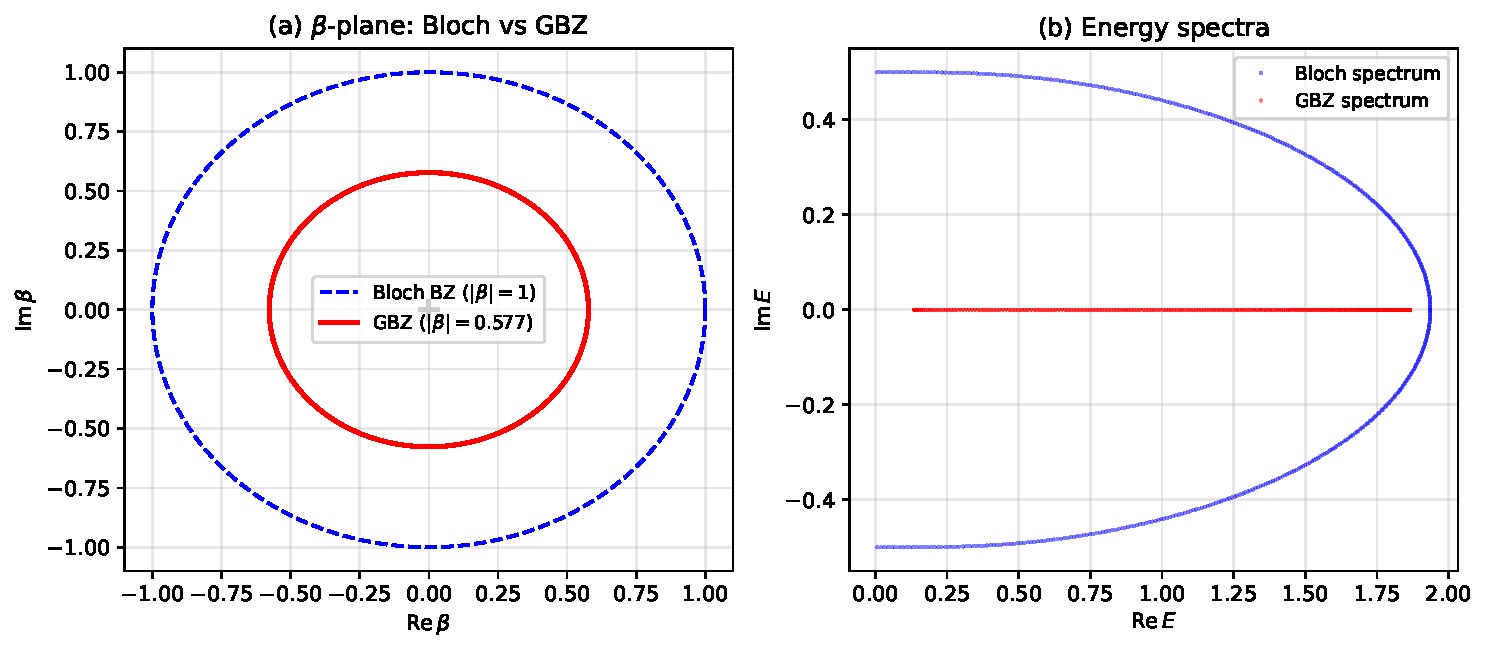
\includegraphics[width=0.85\linewidth]{figures/fig_f14_gbz_construction.pdf}
 \caption{Generalized Brillouin zone (GBZ) for an asymmetric-hopping
 Hatano--Nelson model with $t_R/t_L=3$.
 (a)~In the $\beta$-plane, the Bloch BZ (blue dashed, $|\beta| = 1$)
 and the GBZ (red solid, $|\beta| = \sqrt{t_L/t_R} \approx 0.577$)
 are concentric circles. The GBZ radius is smaller than unity,
 reflecting the exponential skin-effect localisation of all bulk
 eigenstates toward one boundary.
 (b)~The energy spectrum computed on the GBZ (red) differs
 qualitatively from the Bloch spectrum (blue), correctly reproducing
 the OBC spectrum and the non-Bloch phase boundary.}
 \label{fig:gbz-construction}
\end{figure}

Evaluating the
band structure on this circle gives
\begin{equation}
 E_{\mathrm{GBZ}}(\theta) = t_R r_{\mathrm{GBZ}}\,e^{i\theta}
 + t_L\,\frac{e^{-i\theta}}{r_{\mathrm{GBZ}}}
 = 2\sqrt{t_R t_L}\,\cos\theta,
 \label{eq:hn-gbz-bands}
\end{equation}
which is exactly the OBC spectrum. The non-Bloch band theory recovers
the correct open-boundary spectrum from the deformed Brillouin zone.

The GBZ radius also fixes the skin envelope.  For amplitudes,
\begin{equation}
  \xi_{\mathrm{amp}} = \frac{1}{|\ln r_{\mathrm{GBZ}}|}
  = \frac{2}{\ln(t_R/t_L)},
  \label{eq:hn-amplitude-length}
\end{equation}
whereas an intensity fit gives
$\xi_{\mathrm{int}}=\xi_{\mathrm{amp}}/2=1/\ln(t_R/t_L)$.  This resolves
the apparent factor-of-two ambiguity: the GBZ radius describes the field
amplitude, while many numerical and experimental plots fit intensity.

\paragraph{Worked numerical example.}
Set $t_R = 1.5$ and $t_L = 0.5$, so that $t_R/t_L = 3$. The PBC
spectrum~\eqref{eq:hn-pbc-spectrum} is an ellipse with semi-major axis
$t_R + t_L = 2.0$ and semi-minor axis $|t_R - t_L| = 1.0$. The spectral
winding number around the origin is $\wnum = +1$, predicting the skin
effect. The OBC spectrum collapses onto the real interval
$[-2\sqrt{0.75},\; 2\sqrt{0.75}] \approx [-1.732,\; 1.732]$. The GBZ
radius is $r_{\mathrm{GBZ}} = \sqrt{1/3} \approx 0.577$, giving a
skin decay constant $\kappa_{\mathrm{skin}} = |\ln r_{\mathrm{GBZ}}|
= \ln\sqrt{3} \approx 0.549$ per site.  The amplitude localization
length is therefore $\xi_{\mathrm{amp}}\approx 1.82$ sites, while an
intensity fit gives $\xi_{\mathrm{int}}\approx 0.91$ sites. For a chain
of $L = 40$ sites,
numerical diagonalisation gives a mean eigenmode centre of mass
$\bar{n} \approx 1.8$, far from the Hermitian bulk value of $20.5$;
the imaginary gauge field $A_{\mathrm{imag}} = i\kappa_{\mathrm{skin}}
\approx 0.549i$ per lattice constant captures this accumulation exactly.

This example is deliberately extreme ($t_R/t_L = 3$) to make the skin
effect visible in a short chain. In photonic realisations the asymmetry is
typically smaller ($t_R/t_L \lesssim 2$), but the localization is still
measurable over chains of 10--20 resonators.

\begin{figure}[t]
 \centering
 
\includegraphics[width=0.58\textwidth]{fig_f14_gbz.pdf}
 \caption{The generalized Brillouin zone deforms the ordinary unit
 circle in the complex $\beta=e^{ik}$ plane. For the Hatano--Nelson
 chain with asymmetric hopping, the GBZ is the circle
 $|\beta|=\sqrt{t_L/t_R}$, which encodes the exponential envelope of
 the open-boundary eigenstates.}
 \label{fig:gbz-circle}
\end{figure}


%% ================================================================
\section{The generalized Brillouin zone: general theory}
\label{sec:gbz}

\subsection{From Bloch to non-Bloch}
\label{ssec:non-bloch}

In the conventional Bloch theory, the wave vector $k$ is real and the
Bloch phase $\beta = e^{ik}$ traces the unit circle $|\beta| = 1$ as
$k$ sweeps the BZ. The energy bands $\omega(k)$ are functions of this
real $k$.

For a non-Hermitian system with the skin effect, the correct ansatz for
the spatial dependence is $\psi_n \propto \beta^n$ with $|\beta| \neq 1$.
The appropriate contour for $\beta$ in the complex plane is the
\emph{generalized Brillouin zone} (GBZ), defined as the locus of
$\beta$ values that satisfy the bulk equation and the open-boundary
condition simultaneously.

\subsection{Construction of the GBZ}
\label{ssec:gbz-construction}

For a system with transfer matrix $\Tmat(\omega, \beta)$, the
characteristic equation
\begin{equation}
 \det[\Tmat(\omega, \beta) - \mathbf{I}] = 0
 \label{eq:characteristic}
\end{equation}
yields $2n$ solutions $\beta_1, \beta_2, \ldots, \beta_{2n}$ (for an
$n$-band model) at each complex frequency $\omega$. Ordering them by
modulus, $|\beta_1| \le |\beta_2| \le \cdots \le |\beta_{2n}|$, the GBZ
is defined by the condition
\begin{equation}
 |\beta_n| = |\beta_{n+1}|.
 \label{eq:gbz-condition}
\end{equation}
This condition ensures that the $n$-th and $(n+1)$-th solutions have
equal decay rates, which is necessary for the boundary conditions at both
ends of an open chain to be satisfied simultaneously.

\subsection{Geometry of the GBZ}
\label{ssec:gbz-geometry}

The GBZ is generically a closed curve in the complex $\beta$ plane,
but it need not be a circle. For the Hatano--Nelson model the GBZ is
the circle $|\beta| = r_{\mathrm{GBZ}}$
(Section~\ref{ssec:hn-gbz}), but richer models produce richer
contours. As the system approaches the Hermitian limit
($t_R \to t_L$), the GBZ smoothly deforms back to the unit circle,
recovering Bloch theory.

\paragraph{NH SSH model: a two-band example.}
The non-Hermitian SSH model has two sublattices per unit cell, with
the Bloch Hamiltonian
\begin{equation}
 H(\beta) = \begin{pmatrix}
 0 & t_1 + t_2/\beta \\
 t_1' + t_2'\,\beta & 0
 \end{pmatrix},
 \label{eq:nhssh-bloch}
\end{equation}
where $t_1, t_2$ are intra- and inter-cell hoppings for the
forward-going off-diagonal element and $t_1', t_2'$ for the
backward-going one. Non-Hermiticity enters whenever $t_1 \neq t_1'$
or $t_2 \neq t_2'$. The energy eigenvalues are
\begin{equation}
 E^2(\beta) = (t_1 + t_2/\beta)(t_1' + t_2'\,\beta).
 \label{eq:nhssh-energy}
\end{equation}
This is a Laurent polynomial in $\beta$; expanding gives a quartic
equation in $\beta$ at fixed $E$, yielding four roots
$\beta_1, \ldots, \beta_4$ ordered by modulus. The GBZ condition
$|\beta_2| = |\beta_3|$ (the middle pair for a two-band model) defines
the GBZ contour.

For the symmetric case $t_1 = t_1' = t$ and
$t_2 = t_2' \equiv s$ (the Hermitian SSH model), the four roots
satisfy $|\beta_1| \le |\beta_2| = |\beta_3| \le |\beta_4|$ on the
unit circle, recovering the standard BZ. But when
$t_2 \neq t_2'$---for instance $t_2 = t_2' + \delta$ with $\delta$
parameterising the asymmetry---the GBZ deforms into a non-circular
closed curve. Near the exceptional points of the band structure,
the contour develops cusps where the two middle roots collide in
both modulus and phase.

The physical content of the GBZ shape is transparent: the deviation
of $|\beta|$ from unity at each point on the GBZ measures the local
skin-mode decay rate. Regions of the GBZ where $|\beta| < 1$
correspond to modes that decay into the bulk from the left boundary;
regions where $|\beta| > 1$ decay from the right boundary. The
overall bias of the GBZ toward $|\beta| < 1$ or $|\beta| > 1$
determines the direction of the macroscopic skin effect.

\paragraph{Photonic transfer-matrix connection.}
In photonic systems, the GBZ formalism connects directly to the
transfer-matrix method of Chapter~\ref{ch:periodicity}, but an important
caveat is needed. For an ordinary reciprocal one-dimensional stack of
isotropic layers, the $2\times2$ transfer matrix written in the usual
field variables is unimodular even when the refractive indices are
complex. Gain and loss make the half-trace complex, so the Bloch
frequencies and Bloch multipliers can be complex, but this alone does
not produce the Hatano--Nelson skin effect.

The transfer-matrix eigenvalues obey
\begin{equation}
 \beta_{1,2} = \xi \pm \sqrt{\xi^2 - 1},
 \qquad \xi = \tfrac{1}{2}\operatorname{Tr}\Tmat_{\mathrm{cell}},
 \label{eq:photonic-transfer-eigenvalues}
\end{equation}
with $\beta_1\beta_2=1$ for a unimodular reciprocal cell. Inside a stop
band one solution grows while the other decays, as in ordinary evanescent
Bloch theory; this is not by itself an extensive skin effect. To obtain
a photonic GBZ analogous to the Hatano--Nelson model one needs a unit
cell whose effective evolution is non-unimodular or nonreciprocal after
projecting to the modal subspace of interest, for example through
magneto-optical bias, temporal modulation, cascaded gain/loss reservoirs,
or a multi-port network with eliminated channels.

In such an effective model the GBZ radius is determined by the middle
roots of the characteristic equation, just as in
Eq.~\eqref{eq:gbz-condition}, and the skin localisation length is
$\xi_{\mathrm{skin}}=1/|\ln r_{\mathrm{GBZ}}|$. The physical origin is
then a direction-dependent round-trip amplification that cannot be
removed without changing the boundary condition.

\paragraph{Quantitative photonic example.}
Consider an effective coupled-resonator chain engineered to have
$t_R/t_L=1.8$ at $\lambda=1550\;\mathrm{nm}$ with lattice spacing
$a=400\;\mathrm{nm}$. The Hatano--Nelson estimate gives
$r_{\mathrm{GBZ}}=\sqrt{t_L/t_R}\approx0.745$ and an amplitude
localisation length
$\xi_{\mathrm{amp}}=1/|\ln r_{\mathrm{GBZ}}|\approx3.4$ unit cells
($1.4\;\mu\mathrm{m}$). In a finite chain of $L=30$ resonators the
right eigenmodes therefore show a clearly resolvable boundary envelope.
The precise number in a full Maxwell simulation depends on radiation
loss, coupling dispersion, and how the auxiliary channels are eliminated,
but the logarithmic relation between $r_{\mathrm{GBZ}}$ and the field
envelope is the same.

\paragraph{Energy-dependent GBZ.}
An important subtlety is that the GBZ depends on the energy $E$.
At different complex energies, the condition
$|\beta_n| = |\beta_{n+1}|$ is satisfied by different $\beta$ values,
tracing out an energy-dependent contour. The \emph{physical} GBZ
relevant for the OBC spectrum is the union of these contours over the
set of OBC eigenvalues. In practice, one often computes the GBZ at a
reference energy (e.g.\ $E = 0$ for chiral-symmetric models) and uses
it to evaluate topological invariants, but this simplification can
fail when the band structure has a complicated topology in the
$(\beta, E)$ space.

\subsection{Non-Bloch band structure}
\label{ssec:non-bloch-bands}

The \emph{non-Bloch band structure} is obtained by evaluating the
eigenvalues $\omega(\beta)$ on the GBZ contour rather than on the unit
circle:
\begin{equation}
 \omega_n^{\mathrm{OBC}} = \omega_n(\beta)\big|_{\beta \in \mathrm{GBZ}}.
 \label{eq:non-bloch-bands}
\end{equation}
This non-Bloch band structure reproduces the OBC spectrum in the
thermodynamic limit, resolving the discrepancy between PBC and OBC that
signaled the breakdown of conventional Bloch theory.


%% ================================================================
\section{Non-Bloch topological invariants}
\label{sec:non-bloch-invariants}

Topological invariants must be computed on the GBZ, not the conventional
BZ, to correctly predict open-boundary spectra and any protected
boundary modes of a non-Hermitian system.

\subsection{Non-Bloch winding number}
\label{ssec:non-bloch-winding}

For a one-dimensional system with chiral symmetry, the non-Bloch winding
number is
\begin{equation}
 \wnum_{\mathrm{GBZ}} = \frac{1}{2\pi i}
 \oint_{\mathrm{GBZ}}
 \frac{\dd}{\dd\beta}\ln\det[H(\beta)]\;\dd\beta,
 \label{eq:non-bloch-winding}
\end{equation}
where $H(\beta)$ is the Bloch Hamiltonian with $e^{ik}$ replaced by
$\beta$. This invariant correctly predicts the number of topological
zero modes under OBC, in contrast to the conventional winding number
computed on the unit circle.

\subsection{Non-Bloch Chern number}
\label{ssec:non-bloch-chern}

In two dimensions, the non-Bloch Chern number is defined by integrating
the Berry curvature over the GBZ torus (the product of two GBZ contours
for $\beta_x$ and $\beta_y$). When the non-Bloch torus is well defined,
this invariant restores the bulk-boundary correspondence for
two-dimensional non-Hermitian systems with a line gap, predicting the
correct number of chiral edge modes.

\subsection{When GBZ invariants differ from Bloch invariants}
\label{ssec:gbz-vs-bloch}

The GBZ and Bloch invariants can differ whenever the GBZ is not the unit
circle---i.e., whenever the skin effect is present. The discrepancy
is maximized when:
\begin{itemize}
 \item The asymmetry $|t_R/t_L|$ is large (strong skin effect).
 \item The system is near a phase boundary where the Bloch invariant
 changes but the GBZ invariant does not, or vice versa.
 \item The GBZ geometry has cusps or self-intersections that cross
 branch cuts of the Bloch Hamiltonian.
\end{itemize}
In all cases, the GBZ invariant is the quantity that should be compared
with open-boundary spectra and boundary modes.

\begin{takeaway}[Non-Bloch band theory]
In non-Hermitian photonic systems with the skin effect, the conventional
Bloch band structure and Bloch topological invariants give incorrect
predictions for open-boundary physics. The generalized Brillouin zone
and the non-Bloch invariants computed on it restore the bulk-boundary
correspondence and provide a faithful description of the photonic
spectrum and boundary modes.
\end{takeaway}


%% ================================================================
\section{Skin effect in two and higher dimensions}
\label{sec:skin-2d}

The skin effect in higher dimensions is qualitatively richer than in
one dimension~\cite{zhang2022universal}.

\paragraph{Universality.}
In two and higher dimensions, the spectral-area result
(Section~\ref{sec:2d-point-gap}) shows why skin accumulation is generic
in many non-Hermitian models: a PBC spectrum that covers finite area in
the complex plane is highly sensitive to boundary geometry. The precise
skin pattern can depend on sample shape, symmetry, and termination, so
the finite spectral area should be viewed as a diagnostic of boundary
sensitivity rather than as a simple one-dimensional winding number.

\paragraph{Corner skin effect.}
In certain two-dimensional systems, all eigenstates are localised at
\emph{corners} rather than edges. This corner-skin effect is a
higher-order analogue of the one-dimensional skin effect and is
classified by a second-order topological invariant. Physically, it
arises when the spectral winding numbers in the $x$ and $y$ directions
are both nonzero but with the same sign, so that the combined
localisation direction points toward a corner.

\paragraph{Geometry-dependent skin effect.}
Some systems exhibit the skin effect for generic polygon-shaped samples
but not for samples with specific symmetry-related shapes. This
geometry dependence has no analogue in Hermitian physics, where the
spectrum is insensitive to the sample shape in the thermodynamic limit.
The physical origin is that the skin localisation direction is determined
by the spectral winding, which depends on the boundary orientation;
different facets of a polygon can have different winding numbers, leading
to competing localisation directions.

\paragraph{Scale-free skin effect.}
A recently discovered variant, the scale-free skin effect, features
localisation lengths that grow with the system size $L$ rather than
remaining fixed. In these systems, the spectrum is sensitive to boundary
conditions at \emph{every} scale, not just in the thermodynamic limit.
The GBZ approaches the unit circle algebraically rather than
exponentially as $L \to \infty$, leading to a non-extensive but still
macroscopic accumulation of states at the boundary.


%% ================================================================
\section{Photonic skin effect}
\label{sec:photonic-skin}

The skin effect has been proposed and observed in several photonic
platforms:

\paragraph{Coupled-resonator optical waveguides.}
Arrays of microring resonators with engineered asymmetric coupling
realise one-dimensional non-Hermitian lattices with tunable skin
effect. The asymmetry is introduced by auxiliary gain/loss elements
or by directional couplers. The key experimental signature is that
light injected at any point in the array propagates preferentially
toward one end, regardless of the injection site.

\paragraph{Photonic mesh lattices: a concrete platform.}
Fibre-loop networks provide a versatile time-multiplexed platform for
studying the skin effect. Two fibre loops of slightly different lengths
create a discrete time-mesh lattice that is isomorphic to a 1+1D
waveguide array. Pulses circulate through the loops, accumulating
nonlinear phase from erbium-doped fibre amplifiers (EDFAs) that provide
controlled gain, while attenuators provide controlled loss. The discrete
time steps map to spatial sites, and the gain/loss can be tuned
independently at each effective site.

Concretely, a mesh lattice with $N = 20$ time slots and asymmetric
coupling ratio $|t_R/t_L| \approx 1.8$ is expected to show a skin
localization length $\xi \approx 1/\ln(1.8) \approx 1.7$ sites. The
experimental signature is a measurement of the output pulse intensity
profile after many round trips: regardless of which time slot receives
the initial pulse, the steady-state intensity peaks at the same boundary
slot. This has been observed in photonic mesh lattices using coupled
fibre loops with balanced gain and loss~\cite{wimmer2015observation},
where the pulse dynamics directly map to the Hatano--Nelson model with
tunable $t_R/t_L$.

\paragraph{Photonic crystals with exceptional points.}
Stable exceptional points in a two-dimensional photonic band structure
often come with complex spectral images of finite area, and this finite
area is a strong warning that boundary-sensitive spectra may appear
under open boundaries~\cite{zhang2022universal}. This connects two
seemingly different non-Hermitian phenomena---EPs and the skin
effect---through the geometry of the PBC spectrum. A concrete prediction
of the skin localization length, however, still requires the non-Bloch
or transfer-matrix analysis for the chosen sample termination.

\paragraph{Non-reciprocal photonic lattices.}
Lattices of waveguides with magneto-optical or time-modulated elements
provide a direct realisation of non-reciprocal hopping, the most
straightforward route to the skin effect. In a magneto-optical
implementation, the Faraday rotation introduces a direction-dependent
phase shift that maps onto asymmetric hopping in the effective
tight-binding model. The resulting skin-effect strength is controlled
by the applied magnetic field, providing a continuously tunable knob.

\paragraph{Experimental signatures.}
The photonic skin effect has three principal experimental signatures
that distinguish it from ordinary boundary-condition sensitivity:
\begin{enumerate}
 \item \textbf{Unidirectional funnelling:} light injected at any site
 propagates to the same boundary, regardless of injection position.
 \item \textbf{Spectral collapse:} the measured transmission spectrum
 under OBC is much narrower than under PBC (e.g., by
 wrapping the array into a ring).
 \item \textbf{Eigenstate tomography:} the intensity profile of each
 resonance shows exponential decay away from one boundary, with a
 decay length that matches the GBZ prediction $\xi = 1/|\ln r_{\mathrm{GBZ}}|$.
\end{enumerate}

\begin{remark}
The photonic skin effect has practical implications for the design of
photonic devices: light in a skin-effect
system accumulates at one boundary regardless of where it is injected,
providing a mechanism for directional transport and amplification that
is topologically robust. This directional funneling effect could be
harnessed for energy harvesting, signal routing, and non-reciprocal
photonic circuits.
\end{remark}


%% ================================================================
\section{Critical non-Hermitian skin effect}
\label{sec:critical-skin}

When two subsystems with different skin-effect localization lengths are
coupled, a new critical behavior emerges~\cite{li2020critical}: the
spectrum and eigenstates exhibit a \emph{discontinuous} jump in the
thermodynamic limit, depending on the order in which the system size
and the coupling strength are taken to their limiting values. This
\emph{critical NHSE} is a phase transition with no Hermitian analogue,
and it highlights the extreme sensitivity of non-Hermitian systems to
boundary conditions and inter-subsystem coupling.

\paragraph{Mechanism.}
Consider two Hatano--Nelson chains with different asymmetry ratios
$t_R^{(1)}/t_L^{(1)} \neq t_R^{(2)}/t_L^{(2)}$, coupled by a hopping
$\kappa$ at a single junction. When $\kappa = 0$, each chain has its
own GBZ radius and its own skin localisation direction. When
$\kappa \neq 0$, the two GBZs must merge into a single contour that
satisfies the combined boundary conditions. The critical NHSE appears
when the two individual GBZ radii are on opposite sides of the unit
circle ($r_1 < 1$ and $r_2 > 1$): the merged GBZ undergoes a
topological transition as a function of $\kappa/t$, jumping
discontinuously from one contour to another at a critical coupling
strength. This discontinuity is reflected in a sudden change of the
OBC spectrum and the localisation pattern of the eigenstates.

\paragraph{Photonic realisation.}
A photonic version of the critical NHSE can be implemented in a
coupled-resonator array where two segments have different gain/loss
profiles, joined at a single coupling point. The coupling strength
$\kappa$ is controlled by the gap between the two resonator segments,
providing a continuously tunable parameter that drives the critical
transition.


%% ================================================================
\section{Connection to earlier chapters}
\label{sec:skin-connections}

The skin effect ties together several threads from earlier chapters:
\begin{itemize}
 \item \textbf{QNMs and open boundaries}
 (Chapter~\ref{ch:qnm}): the spatial divergence of QNM fields
 is a single-resonator version of the skin effect. In a periodic
 system, the skin effect is the collective version: every Bloch state
 acquires a QNM-like exponential envelope.
\item \textbf{Point-gap topology}
 (Chapter~\ref{ch:point-gap}): the winding number that classifies
 point-gap phases diagnoses boundary-sensitive spectra. In one
 dimension, a nonzero point-gap winding means the PBC and OBC spectra
 differ, and the GBZ is needed.
 \item \textbf{Poles and zeros}
 (Chapter~\ref{ch:poles-zeros}): the poles of the scattering
 matrix of a finite non-Hermitian chain are the OBC eigenvalues.
 The spectral collapse from PBC loops to OBC arcs is a statement
 about the pole motion under boundary-condition changes.
 \item \textbf{Bulk-boundary correspondence}
 (Chapter~\ref{ch:bbc-rebuilt}): the skin effect forces a
 reconstruction of the BBC. The next chapter develops this
 reconstruction using the GBZ and the non-Bloch invariants
 introduced here.
\end{itemize}

\subsection{From Maxwell transfer matrices to the photonic GBZ}
\label{ssec:maxwell-gbz}

The GBZ construction above uses tight-binding language, but it extends
naturally to the full Maxwell formalism via the transfer-matrix method
of Chapter~\ref{ch:boundaries}. For a one-dimensional photonic crystal
with $N$ bilayers, each described by a $2\times 2$ transfer matrix
$\mathbf{M}(\omega)$, the Bloch condition is
$\mathbf{M}(\omega)\,\mathbf{v} = \beta\,\mathbf{v}$, where $\beta = e^{iKd}$ is the
Bloch phase per unit cell. The two eigenvalues $\beta_1(\omega)$ and
$\beta_2(\omega)$ of $\mathbf{M}$ satisfy $\beta_1\beta_2 = \det\mathbf{M}$.
In the Hermitian case, $|\det\mathbf{M}| = 1$ and the two eigenvalues are
reciprocal partners on the unit circle in a pass band. For a reciprocal
lossy stack, $\det\mathbf{M}$ can still equal unity even though the
trace is complex; the eigenvalues then move off the unit circle as
ordinary growing/decaying Bloch multipliers, not automatically as a
skin-effect GBZ.

The photonic GBZ is constructed by the same procedure as in the
tight-binding case:
\begin{enumerate}
 \item Compute $\beta_1(\omega)$ and $\beta_2(\omega)$ from the
 transfer matrix at each complex frequency $\omega$.
 \item The GBZ contour is the locus of $\beta$ values where
 $|\beta_1| = |\beta_2|$.
 \item The non-Bloch band structure is obtained by evaluating
 $\omega(\beta)$ on this contour.
\end{enumerate}
For a concrete gain/loss photonic crystal with bilayer permittivities
$\varepsilon_A = 4 + 0.3i$ and $\varepsilon_B = 4 - 0.3i$, the
transfer-matrix eigenvalues deviate from the unit circle in stop bands
and the complex band structure can form loops. To claim a skin effect,
one must additionally show that the open-boundary spectrum is reproduced
by a GBZ different from the ordinary Bloch contour. In practice this
usually requires an effective nonreciprocal coupling mechanism, a
time-modulated unit cell, or a multi-channel network whose eliminated
channels generate a direction-dependent round-trip gain.
